

\begin{frame}{\ft{Toward a Unified Event Model}}
\section{Event\\Model}
\doubleFrame{\large{One benefit of merging 
image-annotation frameworks is that,  
while the semantic and geometric meaning of 
annotations varies across scientific fields, HCI 
protocols (as annotations are viewed and 
manipulated by users) are largely the same.}}

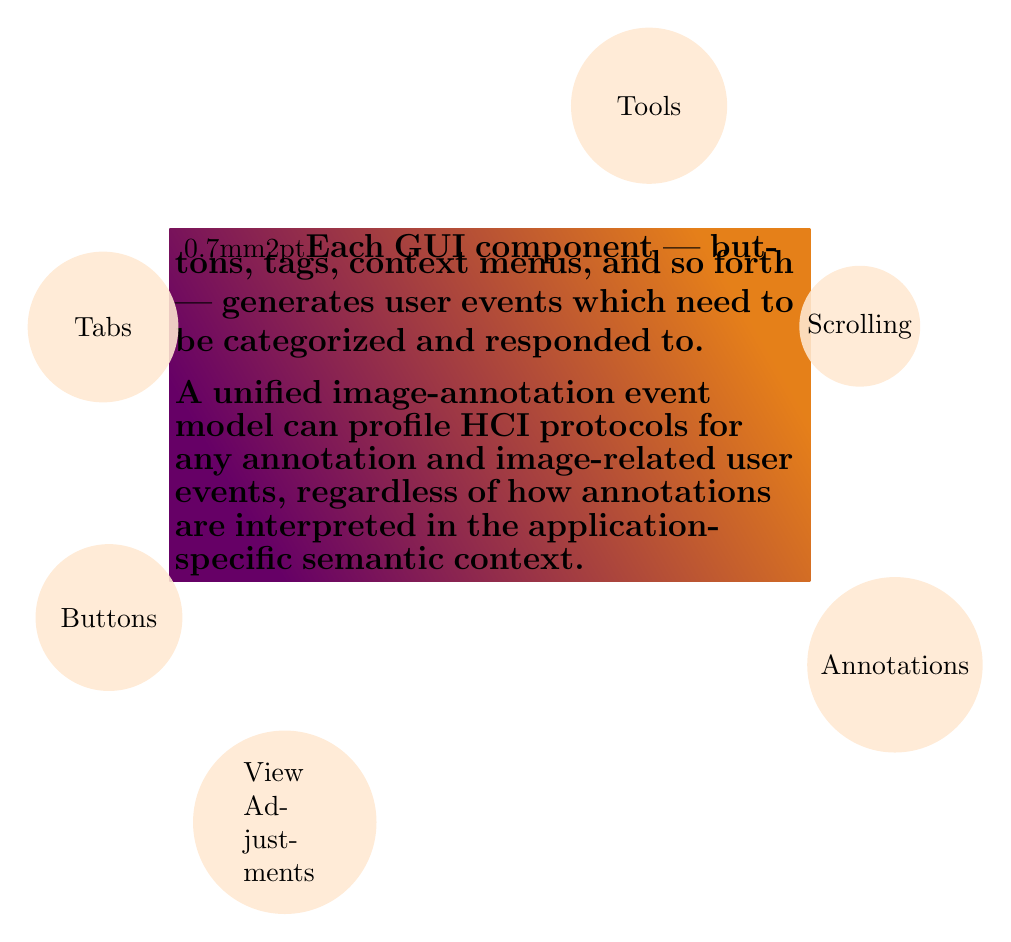
\begin{tikzpicture}
\nodeincludegraphicsTRRS{0.92}{0cm}{0cm}{0cm}{0.2cm}{pics/rad.png}

 \node [anchor=west, bottom color=brown!40!orange,
top color=magenta!40!black, shading angle=120,
inner sep=2, text width=8cm]
  (longnote) at (4.7,10.3) {\vspace{-8pt} %  %{\color{rb!85!red}{
  {\cframedboxx{0.7mm}{2pt}{\large\textbf{Each GUI 
component --- buttons, tags, context menus, and so 
forth --- generates user events 
which need to be categorized and responded to.\vspace{.5em}\\
A unified image-annotation event model can 
profile HCI protocols for any annotation and 
image-related user events, regardless of 
how annotations are interpreted in the 
application-specific semantic context.
}}}};

\node [anchor=west,circle,fill=orange!18!white,inner sep=12, 
opacity=0.88, text opacity=1] (tools) at (9.8, 14.1) {Tools};

\colorarr{>=latex, ->}{fcBoxColor!60!black}
{0.8}{blGreen!30!red}{1}{1mm}{tools.north east}{13.5,16.2}


\node [anchor=west,circle,fill=orange!18!white,inner sep=4, 
opacity=0.88, text opacity=1] (annotations) at (12.8, 7) {Annotations};

\colorarr{>=latex, ->}{fcBoxColor!60!black}
{0.8}{blGreen!30!red}{1}{1mm}{annotations.east}{14.5,8.5}


\node [anchor=west,circle,fill=orange!18!white,inner sep=12, 
opacity=0.88, text opacity=1] (tabs) at (2.9, 11.29) {Tabs};

\colorarr{>=latex, ->}{fcBoxColor!60!black}
{0.8}{blGreen!30!red}{1}{1mm}{tabs.north west}{2,14}


\node [anchor=west,circle,fill=orange!18!white,inner sep=7, 
opacity=0.88, text opacity=1] (buttons) at (3, 7.6) {Buttons};

\colorarr{>=latex, ->}{fcBoxColor!60!black}
{0.8}{blGreen!30!red}{1}{1mm}{buttons.north west}{1.5,10.8}


\node [anchor=west,circle,fill=orange!18!white,inner sep=2, 
opacity=0.88, text opacity=1] (scr) at (12.7, 11.3) {Scrolling};

\colorarr{>=latex, ->}{fcBoxColor!60!black}
{0.8}{blGreen!30!red}{1}{1mm}{scr.north east}{19.7,12.5}


\node [anchor=west,circle,fill=orange!18!white,inner sep=5, 
opacity=0.88, text opacity=1,text width=30pt] (iv) at (5, 5) {View Adjustments};

\colorarr{>=latex, ->}{fcBoxColor!60!black}
{0.8}{blGreen!30!red}{1}{1mm}{iv.south east}{7.8,2.85}


\end{tikzpicture}


\end{frame}

